\documentclass{article}
\usepackage[utf8]{inputenc}
\usepackage{longtable}
\usepackage{gensymb}
\usepackage{graphicx}
\usepackage{siunitx}
\usepackage{caption}
\usepackage[colorlinks,bookmarks=false,citecolor=blue,linkcolor=blue,urlcolor=blue]{hyperref}
\usepackage{relsize}
\usepackage{amsmath}
\usepackage{amssymb}
\usepackage{bm}
\usepackage{multirow}

\begin{document}
\begin{titlepage}
\begin{center}

\includegraphics[scale=0.12]{document/niser.png}
\line(1,0){340}\\
[1mm]
\begin{large}
\textbf{\huge Diffraction of Light \\ \normalsize using Single and Double Slit}\\ 
\end{large}
\line(1,0){200}\\
[5cm]
\large MAITREY SHARMA\\
\small (1911093)\\
[3.5cm]
Third Year Integrated M.Sc.\\
\textbf{School of Physical Sciences}\\
\textbf{National Institute of Science Education and Research, Bhubaneshwar}\\
\small September 14, 2021
\end{center} 
\end{titlepage}
\newpage
\section{Aim}
\begin{itemize}
    \item To determine the wavelength of laser light from single-slit diffraction pattern.
    \item To determine the thickness of a fine wire from its diffraction pattern. 
    \item Compare the thickness of the wire with the single-slit width that form the same diffraction pattern as wire and hence verify the Babinet’s principle.
    \item To understand the diffraction pattern due to double slit and determine the slit width and the opaque gap between the two slits.
\end{itemize}
\section{Apparatus}
\begin{enumerate}
    \item Laser source (and safety goggles),
    \item Screen and a ruled-paper for measurement,
    \item A thin-wire,
    \item Variable single-slit and double-slit,
    \item Measuring tape,
    \item A travelling microscope and a digital camera.
\end{enumerate}

\section{Introduction}
\noindent \textbf{Diffraction} refers to various phenomena that occur when a wave encounters an obstacle or opening. It is defined as the bending of waves around the corners of an obstacle or through an aperture into the region of geometrical shadow of the obstacle/aperture. The diffracting object or aperture effectively becomes a secondary source of the propagating wave. When light passes through a small opening or around an edge, secondary waves from different portions of the emerging wavefront will, in general, travel different distances before reaching a screen. Although the waves from secondary sources are all in phase to start with, they will be out of phase by the time they reach the screen. The interference of these radiation emitted by secondary wavefront leads to the phenomenon of diffraction.
\par
\noindent
The diffraction phenomena are usually divided into two categories: \textbf{\textit{Fresnel diffraction}} and \textbf{\textit{Fraunhofer diffraction}}. In the Fresnel class of diffraction the source of light and the screen are, in general, at a finite distance from the diffracting aperture (see figure \ref{fig:fraun&fresnel} (a)). In the Fraunhofer class of diffraction, the source and the screen are at infinite distances from the aperture; this is easily achieved by placing the source on the focal plane of a convex lens and placing the screen on the focal plane of another convex lens (see figure \ref{fig:fraun&fresnel} (b)).
\clearpage
\begin{figure}[h!]
    \centering
    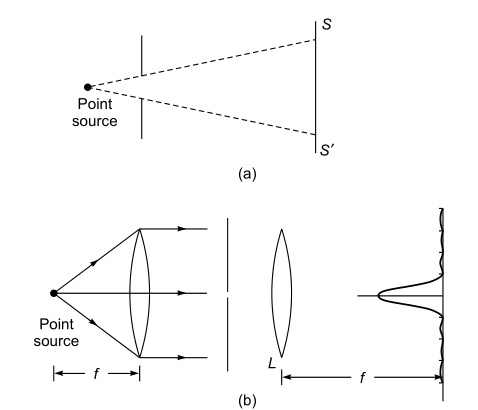
\includegraphics[scale = 0.85]{Figures/fraun&fresnel.png}
    \captionsetup{justification=centering}
    \caption{(a) When either the source or the screen (or both) is at a finite distance from the aperture, the diffraction pattern corresponds to the Fresnel class. (b) In the Fraunhofer class both the source and the screen are at infinity.}
    \label{fig:fraun&fresnel}
\end{figure}
\par
\noindent
In this experiment, our study will be limited to the Fraunhofer class of diffraction.
\par
\noindent
The \textbf{\textit{Babinet's principle}} states that the diffraction pattern from an opaque body is identical to that from a hole of the same size and shape except for the overall forward beam intensity. The fact that Fraunhofer diffraction pattern due to an obstacle is virtually 
identical to that of an opening of same dimension is an example of a general rule called 
Babinet's principle. This principle can be verified by replacing once again the wire with a 
single- slit and varying the slit-width until the pattern matches exactly. The slit width can then 
be compared with the wire thickness. 

\section{Schematics and Setup}
\noindent
The following figures present the outline diagrams and schematics of the the two modes of Fraunhofer diffraction we will be studying in this experiment, along with the experimental setup of the apparatus.
\begin{figure}
    \centering
    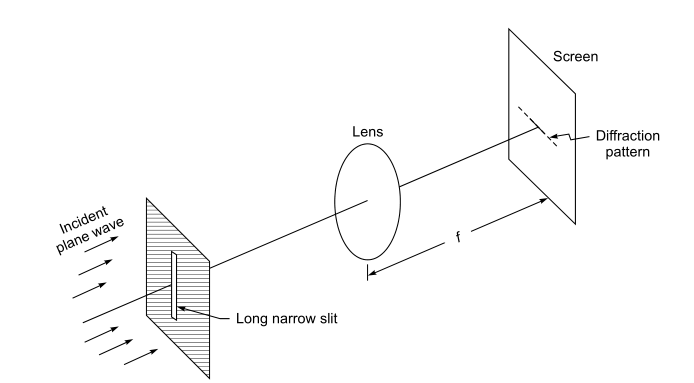
\includegraphics[scale = 0.65]{Figures/singleslit.png}
    \captionsetup{justification=centering}
    \caption{Diffraction of a plane wave incident normally on a long narrow slit of width $b$. Notice that the spreading occurs along the width of the slit.}
    \label{fig:snglslit}
\end{figure}

\begin{figure}
    \centering
    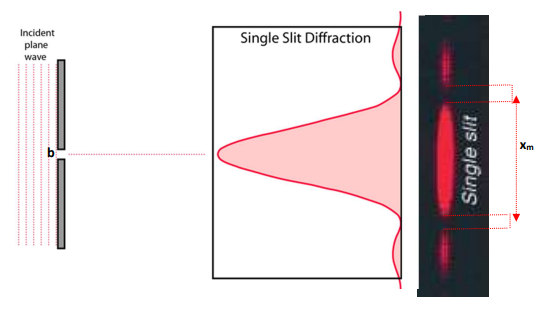
\includegraphics[scale = 0.75]{Figures/snglschematics.png}
    \captionsetup{justification=centering}
    \caption{Schematics for single-slit diffraction. Distance between minima $x_m$ is calculated from the average minima position on either side of principal maxima.}
    \label{fig:snglschem}
\end{figure}
\begin{figure}
    \centering
    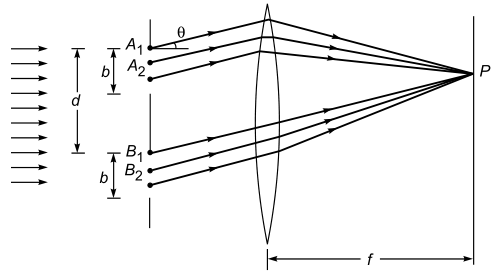
\includegraphics[scale = 0.65]{Figures/doubleslit.png}
    \captionsetup{justification=centering}
    \caption{Fraunhofer diffraction of a plane wave incident normally on a double slit.}
    \label{fig:dblslit}
\end{figure}
\begin{figure}
    \centering
    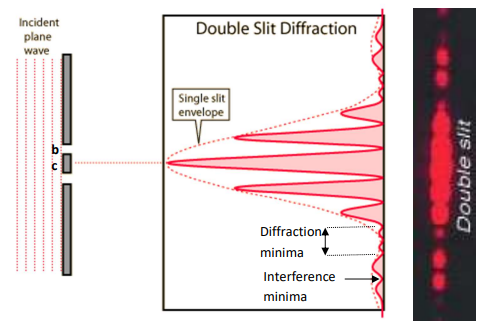
\includegraphics[scale = 0.75]{Figures/dblschematics.png}
    \captionsetup{justification=centering}
    \caption{Schematics for Double-slit diffraction}
    \label{fig:dblschem}
\end{figure}

\begin{figure}[h!]
    \centering
    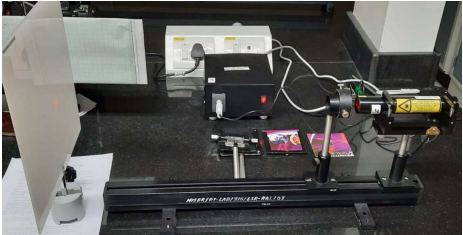
\includegraphics[scale = 0.95]{Figures/setup.png}
    \captionsetup{justification=centering}
    \caption{Setup with Laser as the source}
    \label{fig:setup}
\end{figure}


\section{Theory}
\noindent When a light of wavelength $\lambda$ is incident normally on a narrow slit of width $b$ as shown in figure (\ref{fig:snglschem}), the resultant intensity of the transmitted light is given by,
\begin{equation}
\label{eq1}
    I = I_0 \dfrac{\sin^2 \beta}{\beta^2}
\end{equation}
with $\beta$,
\begin{center}
    $\beta = \dfrac{\pi b \sin \theta}{\lambda}$
\end{center}
\noindent
Here, $\theta$ is the angle of diffraction. The diffraction pattern consists of a principal maximum 
for $\beta = 0$, where all the secondary wavelets arrive in phase, and several secondary maxima of 
diminishing intensity with equally spaced points of zero intensity at $\beta = m \pi$. The positions of 
the minima of a single-slit diffraction pattern are given by,
\begin{equation}
    m \lambda = b \sin \theta
\end{equation}
for $m = \pm 1, \pm 2, \pm 3 \ldots$.
\par
\noindent
If $\theta$ is small, i.e. the slit to screen distance $D$ is large compared to the distance $x_m$ between two $m^{th}$ order minima (on either side of principal maximum), then
\begin{equation}
\label{eq3}
    \sin \theta \approx \theta = \dfrac{x_m}{2 D} \implies m \lambda = \dfrac{b x_m}{2D}
\end{equation}
\par
\noindent The above equation (\ref{eq3}) can be used to determine the wavelength of the monochromatic light source, laser in this case, by measuring $b$, $D$ and $x_m$ for various $m$. The positions of the 
minima can be obtained by averaging the two extremities of the zero intensity region, as shown 
in figure (\ref{fig:snglschem}). A real photographic image of the pattern is shown in figure (\ref{fig:snglphoto}).

\begin{figure}
    \centering
    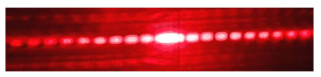
\includegraphics{Figures/snglphoto.png}
    \captionsetup{justification=centering}
    \caption{Photographic image of a single-slit diffraction pattern}
    \label{fig:snglphoto}
\end{figure}
\par
\noindent
If the single-slit is replaced by a thin wire obstacle, which blocks as much laser light as a 
single-slit will allow to pass, the resulting diffraction pattern will be identical to that of a 
single-slit. Knowing the wavelength $\lambda$ of the laser light, the equation (\ref{eq3}) can be used to 
determine the thickness of the wire $b$ as,
\begin{equation}
\label{eq4}
    b = \dfrac{2 m \lambda D}{x_m}
\end{equation}
A typical diffraction pattern of a wire obstacle is shown in figure (\ref{fig:thinwire}). Here too, the positions of the minima are calculated by averaging the two ends of the spread of zero intensity regions as shown in figure (\ref{fig:snglschem}).
\begin{figure}[h!]
    \centering
    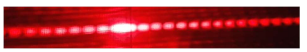
\includegraphics{Figures/thinwire.png}
    \captionsetup{justification=centering}
    \caption{Photographic image of diffraction pattern from a thin wire– similarity with single-slit pattern is what Babinet’s principle asserts.}
    \label{fig:thinwire}
\end{figure}
\par
\noindent
If instead of single-slit, we have two parallel slits each of width $b$ separated by an opaque space 
of width $c$ (figure (\ref{fig:dblschem})), the corresponding intensity distribution of the Fraunhofer pattern formed is given by, 
\begin{equation}
    I - I_0 \dfrac{\sin^2 \beta^2}{\beta^2} \cos^2 \gamma
\end{equation}
$\theta$ being the angle of diffraction. Also,
\begin{center}
    $\beta = \dfrac{\pi b \sin \theta}{\lambda}$, $\gamma = \dfrac{\pi d \sin \theta}{\lambda}$, $d = b + c$
\end{center}
The intensity distribution is a product of two terms: the first term ($\dfrac{\sin^2 \beta^2}{\beta^2}$) represents diffraction pattern produced by single-slit (\ref{eq1}) and the second term ($\cos^2 \gamma$) is the characteristic of interference produced by two beams of equal intensity and phase difference $\gamma$. The overall pattern, therefore, consists of single-slit diffraction fringes each broken into narrow maxima and minima of interference fringe.
\par
\noindent
The minima for the interference fringes are at $\gamma = (2p + 1)\pi/2$ with $p = 0, 1, 2 \ldots$ and those for diffraction fringes are at $\beta = m \pi$ where $m = 1, 2, 3 \ldots$ 
\par
\noindent
The conditions for minima are,
\begin{equation}
    d \sin \theta = (p + \dfrac{1}{2})\lambda
\end{equation}
\begin{equation}
    b \sin \theta = m \lambda
\end{equation}
A photographic image of the double-slit Fraunhofer pattern obtained with laser beam is shown in figure (\ref{fig:dblphoto}).

\begin{figure}[h!]
    \centering
    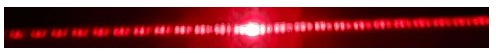
\includegraphics[scale = 0.9]{Figures/dblphoto.png}
    \captionsetup{justification=centering}
    \caption{Photographic image of double-slit diffraction pattern – each diffraction maxima is broken up into interference fringes}
    \label{fig:dblphoto}
\end{figure}
\noindent
As it is evident from the figure (\ref{fig:dblphoto}) that the positions of interference and diffraction minima hardly show any spread at all, it is better to consider differences in positions between $n$ consecutive minima, that is,
\begin{center}
    $\Delta x_p = x_{p+n} - x_p$ and $\Delta x_m = x_{m+n} - x_m$
\end{center}
\noindent
Assuming as before, the distance $D$ of the screen from the double-slit is large compared to $x_p$ and $x_m$, we have, 
\begin{equation}
    \sin \theta \approx \theta = \dfrac{x_p}{D} \implies \boxed{d = \dfrac{n \lambda D}{\Delta x_p}}
\end{equation}
\begin{equation}
    \sin \theta \approx \theta = \dfrac{x_m}{D} \implies \boxed{b = \dfrac{n \lambda D}{\Delta x_m}}
\end{equation}





\section{Observations}
\begin{enumerate}
    \item Least count of vernier callipers = \SI{0.001}{\centi \metre}.
    \item Wavelength, $\lambda = \SI{632.816}{\nano \metre}$.
    \item Slit screen distance, $D = \SI{3.42}{\metre}$.
\end{enumerate}
\clearpage
\begin{table}[h!]
\centering
\caption{\textbf{Determination of $b$ and $c$ using travelling microscope}}
\resizebox{\textwidth}{!}{%
\begin{tabular}{|c|c|c|c|c|c|c|c|c|c|c|}
\hline
\hline
\multirow{2}{*}{\textbf{Object}} &
  \multicolumn{4}{c|}{\textbf{Left Edge}} &
  \multicolumn{4}{c|}{\textbf{Right Edge}} &
  \multirow{2}{*}{\begin{tabular}[c]{@{}c@{}}\textbf{Width}\\ ($\alpha_l - \alpha_r$)\\ (cm)\end{tabular}} &
  \multirow{2}{*}{\begin{tabular}[c]{@{}c@{}}\textbf{\textless{}Width\textgreater}\\ (cm)\end{tabular}} \\ \cline{2-9}
 &
  \begin{tabular}[c]{@{}c@{}}\textbf{M}\\ (cm)\end{tabular} &
  \textbf{V} &
  \begin{tabular}[c]{@{}c@{}}\textbf{T}\\ (cm)\end{tabular} &
  \begin{tabular}[c]{@{}c@{}}\textbf{\textless{}T\textgreater}\\ $\alpha_l$\\ (cm)\end{tabular} &
  \begin{tabular}[c]{@{}c@{}}\textbf{M}\\ (cm)\end{tabular} &
  \textbf{V} &
  \begin{tabular}[c]{@{}c@{}}\textbf{T}\\ (cm)\end{tabular} &
  \begin{tabular}[c]{@{}c@{}}\textbf{\textless{}T\textgreater}\\ $\alpha_r$\\ (cm)\end{tabular} &
   &
   \\ \hline \hline
\multirow{2}{*}{Slit - 1} &
  6.10 &
  8 &
  6.108 &
  \multirow{2}{*}{6.109} &
  6.05 &
  9 &
  6.059 &
  \multirow{2}{*}{6.062} &
  \multirow{2}{*}{0.047} &
  \multirow{4}{*}{$b = 0.048$} \\ \cline{2-4} \cline{6-8}
 &
  6.10 &
  10 &
  6.110 &
   &
  6.05 &
  15 &
  6.065 &
   &
   &
   \\ \cline{1-10}
\multirow{2}{*}{Slit - 2} &
  6.05 &
  5 &
  6.055 &
  \multirow{2}{*}{6.057} &
  6.00 &
  2 &
  6.002 &
  \multirow{2}{*}{6.009} &
  \multirow{2}{*}{0.048} &
   \\ \cline{2-4} \cline{6-8}
 &
  6.05 &
  9 &
  6.059 &
   &
  6.00 &
  15 &
  6.015 &
   &
   &
   \\ \hline
\multirow{2}{*}{\begin{tabular}[c]{@{}c@{}}Slit - 1\\ + wire\end{tabular}} &
  6.10 &
  8 &
  6.108 &
  \multirow{2}{*}{6.109} &
  6.05 &
  5 &
  6.055 &
  \multirow{2}{*}{6.057} &
  \multirow{2}{*}{0.052} &
  \multirow{4}{*}{$d = 0.050$} \\ \cline{2-4} \cline{6-8}
 &
  6.10 &
  10 &
  6.110 &
   &
  6.05 &
  9 &
  6.059 &
   &
   &
   \\ \cline{1-10}
\multirow{2}{*}{\begin{tabular}[c]{@{}c@{}}Slit - 2\\ + wire\end{tabular}} &
  6.05 &
  5 &
  6.055 &
  \multirow{2}{*}{6.057} &
  6.00 &
  2 &
  6.002 &
  \multirow{2}{*}{6.009} &
  \multirow{2}{*}{0.048} &
   \\ \cline{2-4} \cline{6-8}
 &
  6.05 &
  9 &
  6.059 &
   &
  6.00 &
  15 &
  6.015 &
   &
   &
   \\ \hline \hline
\end{tabular}%
}
\end{table}

\begin{center}
    \boxed{\boldmath c = d - b = \SI{0.002}{\centi \metre}}
\end{center}

\begin{table}[h!]
\centering
\caption{\textbf{Determination of $d$ using diffraction pattern}}
\begin{tabular}{|c|c|c|c|c|c|}
\hline
\hline
\multirow{2}{*}{\begin{tabular}[c]{@{}c@{}}\textbf{Interference}\\ \textbf{Order}\\ $p+n$\end{tabular}} &
  \multicolumn{2}{c|}{\textbf{Left fringes}} &
  \multicolumn{2}{c|}{\textbf{Right fringes}} &
  \multirow{2}{*}{\begin{tabular}[c]{@{}c@{}}\textbf{\textless{}$d$\textgreater}\\ (10^{-4}\ m)\end{tabular}} \\ \cline{2-5}
 &
  \begin{tabular}[c]{@{}c@{}}$\Delta x_p$\\ (cm)\end{tabular} &
  \begin{tabular}[c]{@{}c@{}}$d$\\ (10^{-4}\ m)\end{tabular} &
  \begin{tabular}[c]{@{}c@{}}$\Delta x_p$\\ (cm)\end{tabular} &
  \begin{tabular}[c]{@{}c@{}}$d$\\ (10^{-4}\ m)\end{tabular} &
   \\ \hline \hline
$p+4$ & 2.1   & 4.12 & 2.1   & 4.12 & \multirow{5}{*}{4.15} \\ \cline{1-5}
$p+5$ & 2.7   & 4.01 & 2.6   & 4.16 &                       \\ \cline{1-5}
$p+6$ & 3.2   & 4.06 & 3.1   & 4.19 &                       \\ \cline{1-5}
$p+7$ & 3.7   & 4.09 & 3.6   & 4.21 &                       \\ \cline{1-5}
$p+8$ & 4.1   & 4.22 & 4.0   & 4.33 &                       \\ \hline \hline
\end{tabular}
\end{table}


\begin{table}[h!]
\centering
\caption{\textbf{Determination of $b$ using diffraction pattern}}
\begin{tabular}{|c|c|c|c|c|c|}
\hline
\hline
\multirow{2}{*}{\begin{tabular}[c]{@{}c@{}}\textbf{Diffraction}\\ \textbf{Order}\\ $m+n$\end{tabular}} &
  \multicolumn{2}{c|}{\textbf{Left fringes}} &
  \multicolumn{2}{c|}{\textbf{Right fringes}} &
  \multirow{2}{*}{\begin{tabular}[c]{@{}c@{}}\textbf{\textless{}$b$\textgreater}\\ (10^{-4}\ m)\end{tabular}} \\ \cline{2-5}
 &
  \begin{tabular}[c]{@{}c@{}}$\Delta x_m$\\ (cm)\end{tabular} &
  \begin{tabular}[c]{@{}c@{}}$b$\\ (10^{-4}\ m)\end{tabular} &
  \begin{tabular}[c]{@{}c@{}}$\Delta x_m$\\ (cm)\end{tabular} &
  \begin{tabular}[c]{@{}c@{}}$b$\\ (10^{-4}\ m)\end{tabular} &
   \\ \hline \hline
$m+1$ & 0.6 & 3.61 & 0.6 & 3.61 & \multirow{5}{*}{3.47} \\ \cline{1-5}
$m+2$ & 1.3 & 3.33 & 1.2 & 3.61 &                       \\ \cline{1-5}
$m+3$ & 2.0 & 3.25 & 1.9 & 3.42 &                       \\ \cline{1-5}
$m+4$ & 2.6 & 3.33 & 2.5 & 3.46 &                       \\ \cline{1-5}
$m+5$ & 3.1 & 3.49 & 3.0 & 3.61 &                       \\ \hline \hline
\end{tabular}
\end{table}
\begin{center}
    \boxed{\boldmath c = d - b = \SI{0.007}{\centi \metre}}
\end{center}

\section{Error Analysis}
The propagation error in a quantity $Q = a + b$ is given by 
\begin{equation}
\label{eq10}
    \delta Q = \sqrt{(\delta a)^2 + (\delta b)^2}
\end{equation}
The standard deviation is given by, 
\begin{equation}
\label{eq11}
    \sigma = \sqrt{\dfrac{\Sigma (x_i - \mu)^2}{N - 1}}
\end{equation}

    \subsection{Through travelling microscope}
    We have, error in average width ($b$ and $d$) $\alpha_l - \alpha_r = \SI{0.001}{\centi \metre}$ using equation (\ref{eq10}) twice.
    Again applying equation (\ref{eq10}), gives error in c as $\SI{0.001}{\centi \metre}$ after rounding off to most significant digit.
    \subsection{Through diffraction pattern}
    Here, to calculate error, we will use standard deviation of the values of $d$ and $b$. Using equation (\ref{eq10}) and equation (\ref{eq11}), error in c is $\SI{0.001}{\centi \metre}$ after rounding off to most significant digit.
    
    
    
\section{Results and Discussions}
\begin{enumerate}
    \item Using the travelling microscope, the value of $c$ is given by \\$\mathbf{0.002 \pm 0.001 cm}$.
        \begin{figure}[h!]
            \centering
            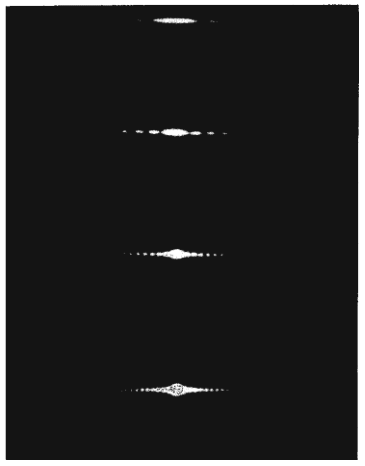
\includegraphics[scale = 0.4]{Figures/snglslitpattern.png}
            \caption{The single-slit diffraction patterns corresponding to $b =$ 0.0088, 0.0176, 0.035, and 0.070 cm, respectively. The wavelength of the light used is $6.328 \times 10^{-5}$ cm.}
            \label{fig:snglpattern}
        \end{figure}
    \item Using the diffraction pattern, the value of $c$ is given by \\$\mathbf{0.007 \pm 0.001 cm}$.
    \item The value of $c$ in case of travelling microscope is found to be close to value obtained through diffraction pattern.
    \item The concept of diffraction is clearly understood through this experiment.
    \item One of the source of this error/ambiguity could be the way readings have been noted.
    \item Some images of diffraction patterns are shown in figures (\ref{fig:snglpattern}) and (\ref{fig:dblpattern}).
        \begin{figure}[h!]
            \centering
            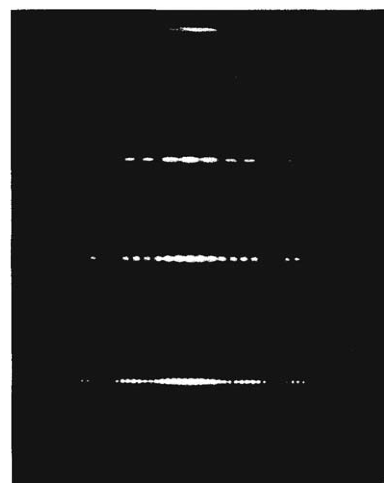
\includegraphics[scale = 0.4]{Figures/dblslitpattern.png}
            \caption{The double-slit Fraunhofer diffraction pattern corresponding to $b =$ 0.0088 cm and $l =$ $6.328 \times 10^{-5}$ cm. The values of $d$ are 0, 0.0176, 0.035, and 0.070 cm, respectively.}
            \label{fig:dblpattern}
        \end{figure}
\end{enumerate}

\section{Precautions}
\begin{enumerate}
    \item The laser beam should not penetrate into eyes as this may damage the eyes permanently.
    \item The laser should be operated at a constant voltage 220V obtainable from a stabilizer. This avoids the flickering of the laser beam.
    \item Keep the laser turned off when not in use.
    \item Do not move the laser around when it is on.
    \item Never aim a laser at another person.
    \item Avoid backlash errors.
\end{enumerate}
\end{document}
